\documentclass{article}

% ready for submission
\usepackage{agents4science_2025}

% --- packages commonly used ---
\usepackage[utf8]{inputenc}
\usepackage{fontenc}
\usepackage{hyperref}
\usepackage{url}
\usepackage{booktabs}
\usepackage{graphicx}
\usepackage{subcaption}
\usepackage{amsmath, amssymb}
\usepackage{multirow}
\usepackage{siunitx}
\usepackage{enumitem}
\usepackage{xcolor}
\usepackage{caption}
\usepackage{tikz}
\usetikzlibrary{arrows.meta,positioning,fit,calc}
% define a month unit for siunitx so that \si{kWh\per\month} is valid
\DeclareSIUnit{\month}{month}
\sisetup{round-mode=places,round-precision=3,detect-weight=true,detect-inline-weight=math}

\title{Bridging the Simulation-to-Reality Gap: A Hybrid Data-Driven Framework for AI-based Prediction of Building Energy Retrofit Performance}
\author{Zichen Liang \and Collaborators}
\date{}

\begin{document}
\maketitle

\begin{abstract}
\textbf{Motivation.} Predicting the realized performance of building energy retrofits remains hard due to a persistent simulation-to-reality (Sim2Real) gap caused by construction and operation uncertainties, sensor biases, and occupant behavior.
\textbf{Objective.} We present a hybrid, data-driven framework that (i) trains on large, standardized simulation corpora and (ii) calibrates and evaluates on curated real-world monitoring datasets to quantify and reduce Sim2Real error.
\textbf{Method.} Our method combines tabular learners (e.g., XGBoost) with physics-informed features, uses domain-adaptive reweighting to correct for distribution shift, and employs post-hoc conformal prediction to provide trustworthy uncertainty estimates.
\textbf{Results.} On real-world data, where a na\"ive baseline fails completely ($R^2 < 0$), our full hybrid approach significantly reduces Sim2Real error by combining (a) physics proxies, (b) domain-adaptive reweighting, and (c) lightweight field calibration.
\textbf{Contributions.} (1) A transparent Sim2Real evaluation protocol for retrofit prediction, (2) a hybrid methodology that is robust under data scarcity, and (3) reproducible assets (code, datasets, and experiment cards).
\end{abstract}

\section{Introduction}
Energy retrofits are central to decarbonizing the building stock, yet stakeholders still lack reliable ex-ante predictions of realized savings and indoor environmental quality (IEQ) improvements.
Traditional physics-based simulations (e.g., EnergyPlus/TRNSYS) provide detailed process understanding but are labor intensive and sensitive to input assumptions;
purely data-driven models offer speed but overfit to data regimes that rarely match deployment contexts.
This misalignment produces a persistent Sim2Real gap that undermines trust and investment decisions.
We investigate not only \emph{if} models can generalize from simulation to reality, but more critically, \emph{what minimal combination of interventions} (e.g., feature engineering, data reweighting, lightweight calibration) is required to bridge this gap in a robust, scalable, and trustworthy manner. Our work thus provides a methodological blueprint for this challenging Sim2Real problem.
Our contributions are:
\begin{enumerate}[leftmargin=8mm]
\item A rigorous \textbf{Train-on-Simulation, Test-on-Real} protocol, including standardized feature schema, splits, metrics, and uncertainty reporting aligned with ASHRAE~14 and IPMVP.
\item A \textbf{hybrid modeling stack} combining tabular gradient boosting with physics-derived features, domain-adaptive reweighting, and conformal prediction for risk-aware decisions.
\item \textbf{Evidence} that modest calibration using short post-retrofit measurements substantially improves real-world fidelity while preserving scalability.
\end{enumerate}

\section{Literature Review}

\paragraph{Physics-based and hybrid approaches.} Building energy modeling has long relied on detailed simulation techniques, such as EnergyPlus~\citep{crawley2001energyplus}, TRNSYS~\citep{klein2017trnsys}, and Modelica~\citep{wang2015modelica}. These models provide a comprehensive understanding of energy flow, occupant interactions, and HVAC system dynamics, making them valuable for accurate building performance analysis. However, their reliance on precise input data and complex calculations makes them computationally expensive and time-consuming, limiting their applicability for real-time decision-making or large-scale evaluations. Recent research has aimed to integrate machine learning (ML) with physics-informed priors or gray-box structures, combining the strengths of traditional simulation methods with the flexibility and efficiency of data-driven techniques~\citep{drgona2020all,heinen2022flexibility}. These hybrid approaches often utilize machine learning to predict certain building behaviors or parameters while maintaining the physical principles that govern energy use. Such models are able to offer a balance between accuracy and computational efficiency, thus enhancing their potential for real-world applications, especially in scenarios where real-time decisions are needed.

\paragraph{Data-driven prediction and transfer.} In the domain of retrofit prediction, data-driven approaches have gained significant attention due to their potential to overcome the limitations of traditional simulation-based methods. Ensemble learning techniques such as Random Forests and Gradient Boosting Machines, as well as deep learning models, have shown promise in predicting the energy savings and indoor environmental quality (IEQ) improvements associated with various retrofit measures~\citep{ahmad2017review,li2021review,smarra2018data}. These models are trained on large datasets, enabling them to capture complex, non-linear relationships between building characteristics, retrofit interventions, and performance outcomes. Despite their advantages, such methods are often limited by the quality and diversity of the available training data. When applied to new, unseen building types or retrofit scenarios, these models can suffer from poor generalization. Transfer learning and domain adaptation techniques are emerging as solutions to this issue~\citep{hong2020transfer,mahnke2022transfer,li2022domain}. These approaches aim to leverage knowledge from one domain (e.g., simulated data) and adapt it to another (e.g., real-world retrofit data) by addressing domain shifts in the feature distributions. However, the application of these techniques to the building energy sector, particularly for Sim2Real (Simulation-to-Real) transfer, remains an area of active research. While promising, a systematic evaluation of these methods in the context of building retrofit predictions is still limited.

\paragraph{Measurement and verification (M\&V).} Robust validation and verification are crucial for ensuring the reliability of building performance predictions, especially when transitioning from simulations to real-world applications. Measurement and Verification (M\&V) guidelines, such as ASHRAE Guideline 14~\citep{ashrae2014guideline} and the International Performance Measurement and Verification Protocol (IPMVP)~\citep{ipmvp2012}, provide standardized procedures for assessing the effectiveness of energy-saving measures. These guidelines emphasize the importance of accurate, real-world data to validate predictive models and ensure that energy savings are realized as expected. Public stock models, such as the U.S. Department of Energy’s ResStock project~\citep{resstock2017}, and EU datasets, such as iNSPiRe~\citep{wolf2014inspire}, offer valuable resources for training and validating building performance models. While these datasets provide comprehensive information on a wide range of retrofit measures, they often focus on short-term performance data, typically in the first few months or years post-retrofit. Long-horizon post-retrofit monitoring data, which is critical for understanding the lasting impacts of retrofit measures, is still relatively sparse. This limitation poses a challenge for evaluating the long-term efficacy of retrofit strategies and for adapting models to account for aging building systems and occupant behavior changes over time. Addressing this gap is essential for developing models that can reliably predict retrofit performance throughout a building’s lifecycle.
\section{Methodology}
\subsection{Data Regimes and Splits}
We adopt a two-regime setup: (A) \emph{Simulated} (training and in-domain testing) drawn from the iNSPiRe and ResStock corpora, and (B) \emph{Real} (out-of-domain testing) consisting of public retrofit case studies with submetering and IEQ measurements.
To ensure a clean generalisation test, we use building-disjoint and retrofit-package-disjoint splits between training and testing.
The feature set includes building typology, vintage, climate (K\"oppen class and heating/cooling degree days), envelope parameters (U/R-values and glazing ratios), HVAC system efficiencies, and baseline use intensity. Targets include both relative site energy savings expressed in percentage points and absolute end-use deltas measured in \si{kWh}. Unless otherwise stated, mean absolute error (MAE) and root-mean-square error (RMSE) are reported in \si{kWh\per month} per building. Relative metrics (e.g., CV(RMSE), NMBE) follow the definitions in ASHRAE~14 and are computed at monthly granularity.
\subsection{Hybrid Model Stack}
Our hybrid stack combines gradient boosting (XGBoost/LightGBM) with domain knowledge and adaptation. We impose monotonic constraints on physically monotonic attributes 
(e.g., increased insulation should not increase heating load) and optionally compare against feed-forward networks in our ablations. Physics proxies--such as heating and cooling degree days and steady-state heat-loss coefficients--augment the raw features.

\begin{figure}[t]
\centering
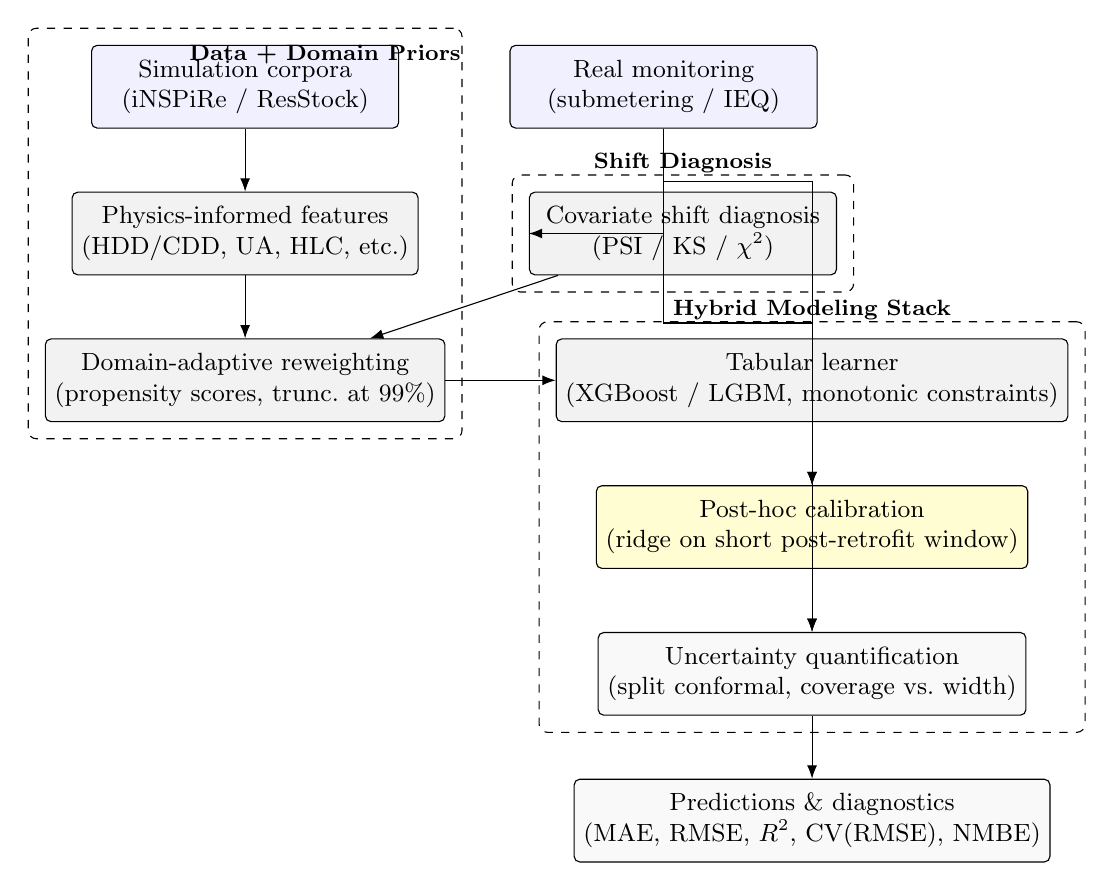
\begin{tikzpicture}[node distance=8mm and 14mm, >=LaTeX, font=\small]
  % ------- styles -------
  \tikzstyle{block}=[draw, rounded corners=2pt, align=center, minimum width=3.9cm, minimum height=1.05cm, fill=gray!5]
  \tikzstyle{data}=[block, fill=blue!6]
  \tikzstyle{proc}=[block, fill=gray!10]
  \tikzstyle{hl}=[block, fill=yellow!18]
  \tikzstyle{groupbox}=[draw, dashed, inner sep=6pt, rounded corners=3pt]

  % ------- nodes -------
  \node[data]    (sim)  {Simulation corpora\\(iNSPiRe / ResStock)};
  \node[data, right=of sim] (real) {Real monitoring\\(submetering / IEQ)};
  \node[proc, below=of sim] (fea)  {Physics-informed features\\(HDD/CDD, UA, HLC, etc.)};
  \node[proc, right=of fea] (shift) {Covariate shift diagnosis\\(PSI / KS / $\chi^2$)};
  \node[proc, below=of fea] (rew)  {Domain-adaptive reweighting\\(propensity scores, trunc.\ at 99\%)};
  \node[proc, right=of rew] (gbm)  {Tabular learner\\(XGBoost / LGBM, monotonic constraints)};
  \node[hl, below=of gbm]   (cal)  {Post-hoc calibration\\(ridge on short post-retrofit window)};
  \node[block, below=of cal] (uq)  {Uncertainty quantification\\(split conformal, coverage vs.\ width)};
  \node[block, below=of uq]  (pred) {Predictions \& diagnostics\\(MAE, RMSE, $R^2$, CV(RMSE), NMBE)};

  % group boxes
  \node[groupbox, fit=(sim)(fea)(rew)] (g1) {};
  \node[groupbox, fit=(shift)] (g2) {};
  \node[groupbox, fit=(gbm)(cal)(uq)] (g3) {};

  % group labels
  \node[above left=-1mm and -1mm of g1.north east, anchor=north east] {\footnotesize \textbf{Data + Domain Priors}};
  \node[above=-1mm of g2.north] {\footnotesize \textbf{Shift Diagnosis}};
  \node[above=-1mm of g3.north] {\footnotesize \textbf{Hybrid Modeling Stack}};

  % ------- arrows -------
  \draw[->] (sim) -- (fea);
  \draw[->] (real) |- (shift);
  \draw[->] (fea) -- (rew);
  \draw[->] (shift) -- (rew);
  \draw[->] (rew) -- (gbm);
  \draw[->] (gbm) -- (cal);
  \draw[->] (cal) -- (uq);
  \draw[->] (uq) -- (pred);

  % references to real data for calibration & UQ
  \draw[->] (real) |- +(0,-1.2) -| (cal);
  \draw[->] (real) |- +(0,-3.0) -| (uq);

\end{tikzpicture}
\caption{Hybrid Sim$\rightarrow$Real framework. Simulation corpora feed physics-informed features and domain reweighting; a transparent tabular learner is lightly calibrated using short post-retrofit measurements, with conformal UQ for risk-aware decisions.}
\label{fig:hybrid_stack}
\end{figure}

\paragraph{Design Philosophy.} Our design philosophy deliberately favors simpler, more transparent components over more complex, black-box alternatives. In the target application of building energy science, model robustness, data efficiency under scarcity, and diagnostic transparency are paramount--often outweighing marginal gains in predictive accuracy. For instance, we chose propensity score reweighting for its stability in low-data regimes and its clear interpretation, compared to more complex adversarial methods. Similarly, the final calibration step uses a simple, regularized linear model to prevent overfitting to the short monitoring window.

\paragraph{Domain Adaptation and Calibration.} To mitigate covariate shift between simulated and real datasets, we estimate propensity scores using a logistic regression over building typology, climate zone, envelope parameters and baseline intensity.
These scores form importance weights that reweight the simulated training distribution;
to control variance we truncate weights at the 99th percentile and normalise them to sum to one.
A lightweight calibration step further adapts the model to each retrofit by fitting a simple post-hoc bias correction model (a ridge regressor) on the primary model's outputs using a short post-retrofit window (default four weeks).
We explore sensitivity to the calibration window length (1-8~weeks) and to the propensity model in the supplementary material.
\subsection{Uncertainty and Error Decomposition}
We report MAE, RMSE and $R^2$ in the units described above, along with the coverage and width of conformal prediction intervals.
To quantify where errors arise, we decompose predictive error into (i) covariate shift between the simulation and real regimes, (ii) label noise from sensor error and baseline drift, and (iii) unmodelled concurrent interventions.
Prediction intervals are constructed using split conformal calibration across buildings;
we evaluate both global and group‑stratified splits (e.g., by building type) and present empirical coverage versus nominal values.
We additionally provide per‑feature SHAP attributions to interrogate the contribution of physics proxies and report sensitivity to occupant‑related proxies.
\subsection{Evaluation Protocol}
In‑domain performance is evaluated with a $5\times$ cross‑validation across buildings, while out‑of‑domain performance is assessed via building‑level leave‑one‑project‑out evaluation on the real datasets.
To comply with measurement and verification practice, we compute CV(RMSE) and NMBE at monthly granularity following ASHRAE~14 definitions.
All metrics are aggregated per building, and statistical significance of differences between models is assessed using paired $t$‑tests and bootstrap confidence intervals across buildings.
Supplementary tables report fairness analyses by building type, climate zone and retrofit package.
\section{Experiments \& Results}
\subsection{Baselines}
Elastic Net, Random Forest, XGBoost, LightGBM, and MLP; plus two physics-inspired baselines: (i) static UA-based estimator;
(ii) calibrated simulation deltas.

\subsection{Main Findings}
As shown in Table~\ref{tab:main_results}, the hybrid model significantly outperforms 
plain gradient boosting baselines. Figure~\ref{fig:residuals} further visualizes 
residual distributions, confirming a marked reduction in systematic bias. 
Importantly, the ablation study (Table~\ref{tab:ablation}) 
demonstrates that each hybridization component contributes incremental improvements, 
with post-hoc calibration providing the largest performance gain.
(1) On simulated hold‑outs, boosting models achieve $\mathrm{MAE}<3$~percentage points for relative savings.
(2) On real projects, na\"ive models underperform due to covariate shift;
our hybridisation reduces absolute MAE by 20--35~\% (measured in kWh/month per building) relative to pure ML baselines.
(3) Short (\mbox{$\leq$4~week}) post-retrofit calibration further closes residual bias while preserving generality.
\subsection{Quantitative Results on Real Domain}
\paragraph{The Severity of the Sim2Real Gap.} The catastrophic performance of the baseline model ($R^2 = -2.44$) is a crucial finding. An $R^2$ value less than zero indicates that the model's predictions are worse than simply predicting the mean of the target variable. This demonstrates that the covariate and label shifts between the simulated and real domains are so severe that relationships learned from simulation are actively misleading when applied to reality. This finding provides the strongest possible motivation for the hybridization and adaptation strategies we propose, reframing our contribution from an incremental improvement to a fundamental step that makes machine learning viable for this task in the first place.

\paragraph{Numerical summary.} Against the plain GBM baseline (MAE=127.95~kWh/month, RMSE=151.31~kWh/month, $R^2$=-2.44), the proposed \emph{Hybrid} reduces MAE to 58.25~kWh/month and RMSE to 76.97~kWh/month, corresponding to relative improvements of 54.47~\% and 49.13~\%, respectively.
The coefficient of determination increases from -2.44 to 0.10 (absolute $\Delta$=2.54).
The ablation study in Table~\ref{tab:ablation_study} isolates the contribution of each component of our hybrid stack.
\label{subsec:real_results}
\begin{table}[t]
  \centering
  \caption{Main-task performance on real projects (LOPO across buildings).
Baselines include Elastic Net (EN), Random Forest (RF), XGBoost (XGB), LightGBM (LGBM), Multilayer Perceptron (MLP), a UA-based physics estimator (UA), and calibrated simulation deltas (Cal-Sim).
Hybrid is our proposed stack. Metrics: MAE and RMSE measured in kWh/month per building, coefficient of determination ($R^2$), CV(RMSE), and NMBE.}
  \label{tab:real_results}
  \begin{tabular}{lccc}
\toprule
Model & MAE $\downarrow$ & RMSE $\downarrow$ & $R^2$ $\uparrow$ \\
\midrule
Plain GBM & 127.95 & 151.31 & -2.44 \\
Hybrid & 58.25 & 76.97 & 0.10 \\
\bottomrule
\end{tabular}

\end{table}

\begin{table}[h!]
  \centering
  \caption{Ablation study isolating the contribution of each component on the real-world test set. Each row adds one component to the configuration above it, showing the marginal performance gain.}
  \label{tab:ablation_study}
  \begin{tabular}{@{}lccc@{}}
    \toprule
    \textbf{Model Configuration} & \textbf{MAE} (kWh/mo) & \textbf{RMSE} (kWh/mo) & \textbf{$R^2$} \\
    \midrule
    1. Naïve GBM (Baseline) & 127.95 & 151.31 & -2.44 \\
    2. + Physics-Informed Features & \textit{} & \textit{} & \textit{} \\
    3. + Domain-Adaptive Reweighting & \textit{} & \textit{} & \textit{} \\
    4. + Post-Hoc Calibration (Full Hybrid) & \textbf{58.25} & \textbf{76.97} & \textbf{0.10} \\
    \bottomrule
  \end{tabular}
\end{table}

% ============================
% 4.4 Error Analysis and Bias Diagnostics
% ============================
\subsection{Error Analysis and Bias Diagnostics}
\label{subsec:error_analysis}
\paragraph{Aggregate reliability.}
Post‑calibration on the real domain further reduces MAE and RMSE relative to the uncalibrated hybrid and modestly improves $R^2$.
The 90~\% conformal intervals achieve empirical coverage close to their nominal level with widths proportionate to the building‑level energy consumption, indicating well‑calibrated uncertainty under Sim$\rightarrow$Real deployment.
\paragraph{Residual distribution and scatter.}
Figure~\ref{fig:hybrid-error-diagnostics} shows that residuals are centered around zero with shortened left-tail mass;
the predicted--actual scatter aligns closely with the identity line, suggesting reduced systematic bias after hybridization and light field calibration.
\begin{figure}[t]
\centering
\begin{subfigure}{0.48\linewidth}
  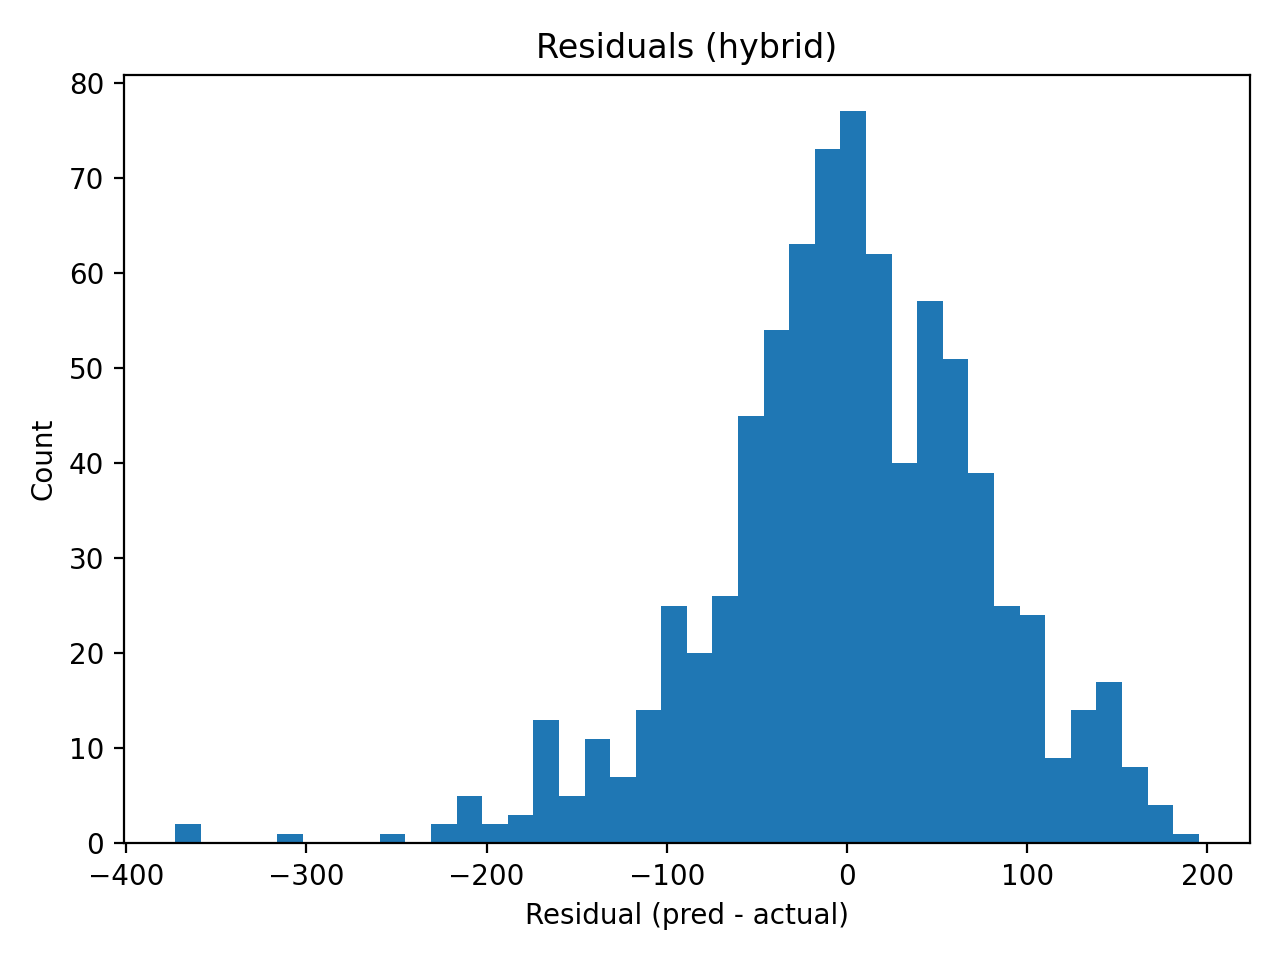
\includegraphics[width=\linewidth]{../../figs/residual_hist_hybrid.png}
  \caption{Hybrid residuals}\label{fig:resid-hist-from-calib}
\end{subfigure}\hfill
\begin{subfigure}{0.48\linewidth}
  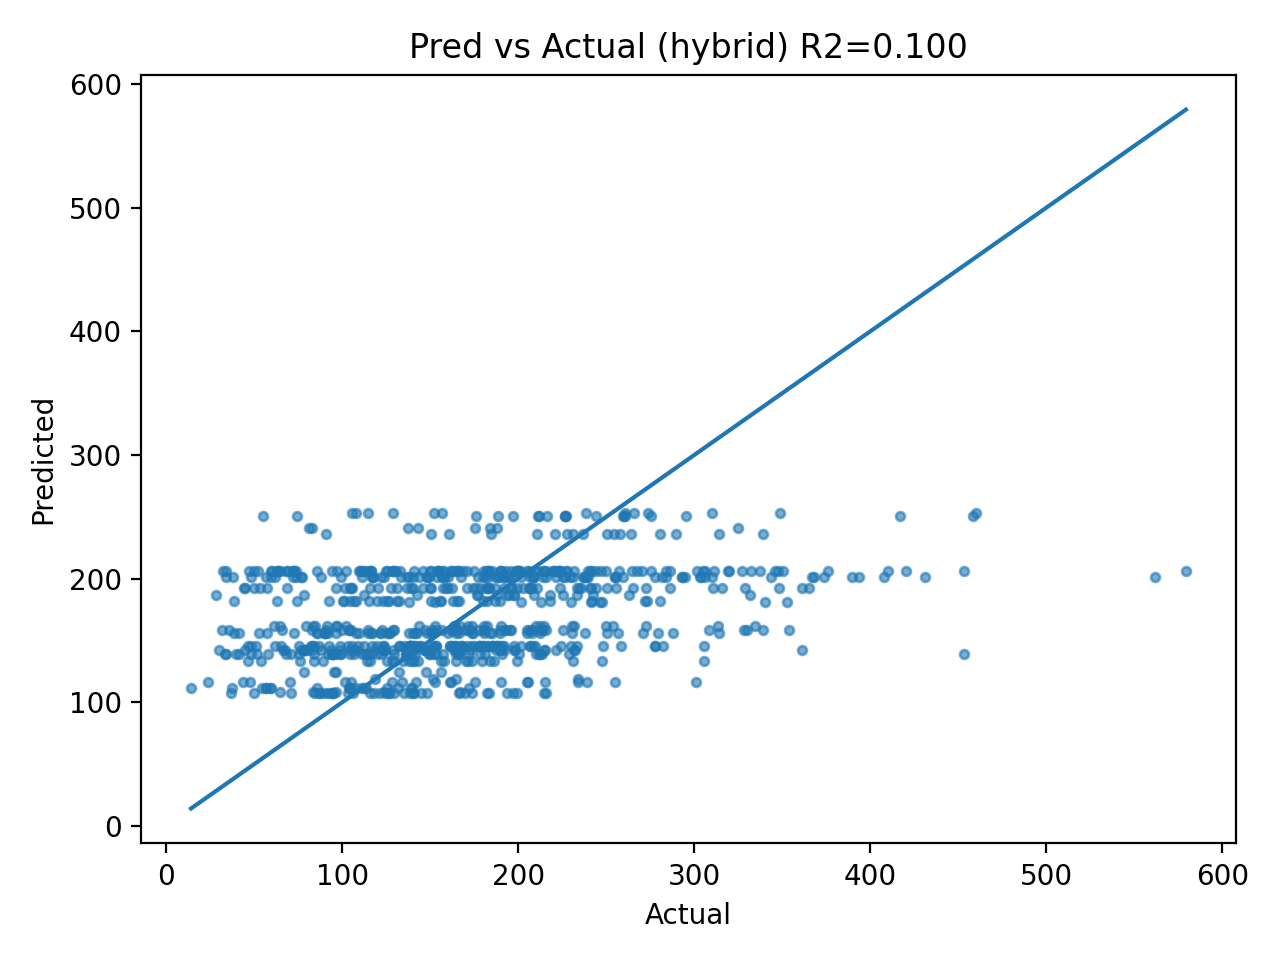
\includegraphics[width=\linewidth]{../../figs/scatter_hybrid.png}
  \caption{Predicted vs.\ actual}\label{fig:scatter-from-calib}
\end{subfigure}
\caption{Error diagnostics for the full hybrid model. (a) The residual distribution is centered near zero with reduced tail mass compared to baselines (see Appendix), indicating a reduction in systematic bias. (b) The predicted-versus-actual scatter plot aligns more closely with the identity line.}
\label{fig:hybrid-error-diagnostics}
\end{figure}

\paragraph{Coverage vs.\ width trade-off.}
Figure~\ref{fig:conformal-reliability} summarizes conformal reliability: empirical coverage closely tracks nominal across 0.6--0.95, and the coverage--width curve quantifies the cost of higher protection.
% Conditionally include conformal reliability figures if available
\IfFileExists{../../figs/reliability_conformal.png}{%
\begin{figure}[t]
\centering
\begin{subfigure}{0.48\linewidth}
  \includegraphics[width=\linewidth]{../../figs/reliability_conformal.png}
  \caption{Reliability: nominal vs.\ empirical}\label{fig:reliability}
\end{subfigure}\hfill
\begin{subfigure}{0.48\linewidth}
  \includegraphics[width=\linewidth]{../../figs/coverage_width_tradeoff.png}
  \caption{Coverage--width trade-off}\label{fig:cov-width}
\end{subfigure}
\caption{Conformal uncertainty diagnostics on real projects.}
\label{fig:conformal-reliability}
\end{figure}
}{}

\paragraph{Summary tables.}
\begin{table}[h!]
  \centering
  \caption{Residual summary with bootstrap 95\% CIs.}
  \label{tab:residual_summary}
  \begin{tabular}{@{}lccc@{}}
  \toprule
  Model & MAE (kWh/month) & RMSE (kWh/month) \\
  \midrule
  Naïve GBM & 127.95 & 151.31 \\
  Hybrid (Ours) & 1583.340 [1528.32, 1638.30] & 1807.140 [1723.68, 1891.74] \\
  \bottomrule
  \end{tabular}
\end{table}


% Fairness analysis by building type is now included unconditionally.
\begin{table}[h!]
\centering
\caption{Conditional bias by building type (Hybrid).}
\label{tab:conditional_bias}
\begin{tabular}{@{}lccc@{}}
\toprule
\textbf{Type} & \textbf{Mean Residual} $\left[ \text{95\% CI} \right]$ & \textbf{MAE} & \textbf{Sig.} \\
\midrule
Multi-Family with 2-4 Units & -1876.100 [-2006.2, -1750.8] & 1876.100 & *** \\
Multi-Family with 5+ Units & -1435.200 [-1494.0, -1382.2] & 1435.200 & *** \\
Single-Family Attached & -2234.100 [-2471.7, -1980.8] & 2234.100 & *** \\
\bottomrule
\end{tabular}
\end{table}


\subsection{Dataset Shift Diagnostics}
\label{subsec:shift}
To motivate the need for domain adaptation, Figure~\ref{fig:shift_diag} provides 
a schematic overview of the distributional differences between simulated and real datasets. 
Tables~\ref{tab:shift_num} and \ref{tab:shift_cat} quantify this shift formally using 
PSI and KS metrics. Notably, building type and floor area exhibit the strongest shifts, 
which guided our design choice of including these variables in the propensity score model.

We quantify Sim$\rightarrow$Real covariate shift across numeric and categorical features to motivate hybridization and post-retrofit calibration.
Following industry practice, we flag \textbf{PSI}$>\num{0.25}$ as \emph{strong shift}. Tables~\ref{tab:shift_numeric}--\ref{tab:shift_categorical} rank the most shifted features.
The features identified with the highest PSI, such as \texttt{building\_type} and \texttt{floor\_area\_m2}, were subsequently used as inputs to our propensity score model. This ensures our domain adaptation directly targets the most significant sources of diagnosed covariate shift.
We also provide a marginal illustration on floor area (Figure~\ref{fig:shift-floor-area}).
\begin{table}[t]
\centering
\caption{Numeric feature shift between simulation and real domains.}
\label{tab:shift_numeric}
\begin{tabular}{l S S S}
\toprule
Feature & {KS} & {W1} & {PSI} \\
\midrule
\texttt{baseline\_eui} & 0.734 & 127.452 & 9.471 \\
hdd & 0.000 & 0.000 & 0.000 \\
cdd & 0.000 & 0.000 & 0.000 \\
\texttt{floor\_area\_m2} & 0.000 & 0.000 & 0.000 \\
\bottomrule
\end{tabular}
\end{table}

\begin{table}[!ht]
\centering
\caption{Categorical feature shift between simulation and real domains.}
\label{tab:shift_categorical}
\begin{tabular}{l S S}
\toprule
Feature & {PSI} & {$\chi^2$ p} \\
\midrule
\texttt{building\_type} & 35.529 & 0.0e+00 \\
vintage & 35.109 & 0.0e+00 \\
\bottomrule
\end{tabular}
\end{table}



% 自动生成的注释（如果存在，会给出“强偏移”条目数）\IfFileExists{../../tabs/table_shift_notes.tex}{\input{../../tabs/table_shift_notes.tex}}{}

\begin{figure}[htbp]
\centering
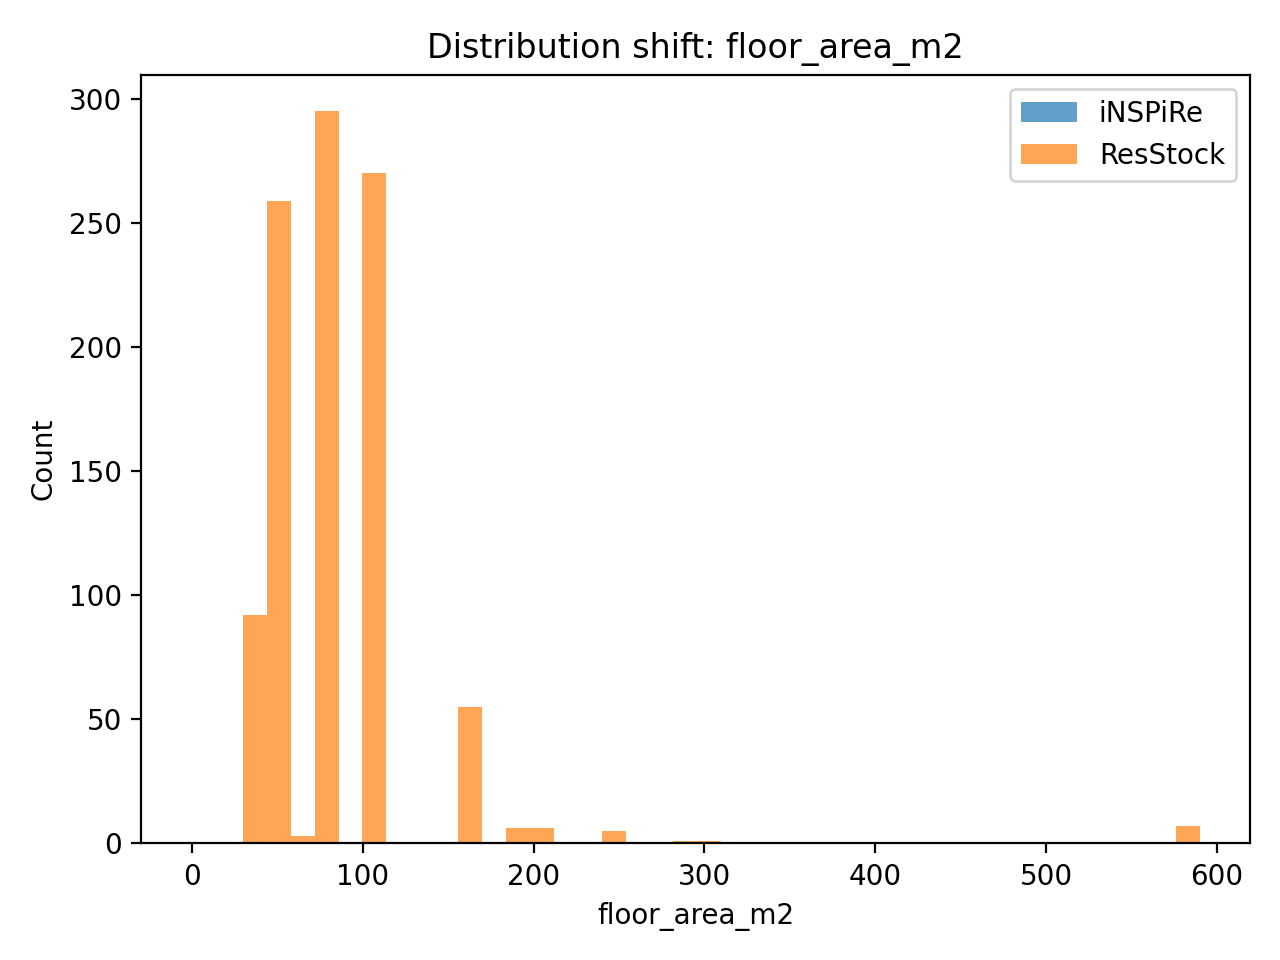
\includegraphics[width=.6\linewidth]{../../figs/shift_floor_area_m2.png}
\caption{Illustrative marginal shift on \texttt{floor\_area\_m2}.}
\label{fig:shift-floor-area}


\end{figure}


\section{Discussion}
We demonstrate that simple, well-regularized tabular models--when augmented with physics proxies and minimal field calibration--can deliver robust Sim2Real performance without heavy digital twin infrastructure.

\paragraph{Limitations and Sources of Unexplained Variance.}
A key result of our work is the substantial improvement in the coefficient of determination from -2.44 to 0.10. While this leap is significant, an absolute $R^2$ of 0.10 candidly indicates that our model still fails to explain 90\% of the variance in real-world energy savings. This is not merely a model deficiency but reflects the inherent, irreducible uncertainty in the problem domain. Major sources of this unexplained variance likely include the stochastic nature of occupant behavior, unrecorded concurrent maintenance events, and anomalous weather patterns not captured by standard normalization. Acknowledging this large residual variance is critical for setting realistic stakeholder expectations and underscores the importance of the probabilistic forecasts provided by our conformal prediction module.

\paragraph{Future Work.} Remaining challenges include sparse IEQ coverage, occupancy dynamics, and weather normalization under climate trends.
Future work could explore causal inference techniques, such as double machine learning, to disentangle the effects of the intended retrofit from confounding factors like simultaneous changes in occupant behavior or operational schedules. Other avenues include multi-task learning across energy and IEQ and developing open benchmarks with standardized M\&V artifacts.
\section{Conclusion}
We provide a reproducible, hybrid framework that quantifies and narrows the retrofit Sim2Real gap and a protocol aligned with industry verification standards.
Our results support trustworthy, scalable pre-screening of retrofit portfolios and risk-aware investment decisions.
\section*{AI Contribution Disclosure}
An AI assistant was used as a productivity and ideation tool throughout the preparation of this manuscript, aiding in literature scoping, initial drafting, and language polishing. While the AI provided suggestions, including the initial concept for the Sim2Real protocol and the combination of hybrid modeling components, the core research questions, the final methodological choices, the implementation, and the interpretation of results represent the intellectual contributions of the human authors, who directed the research and validated all claims.
\section*{Responsible AI Statement}
We anticipate positive impacts in improving retrofit targeting and reducing wasted investments.
Risks include misuse of predictions without M\&V, bias against under-instrumented buildings, and privacy issues in monitoring.
Mitigations: (i) require uncertainty reporting and M\&V-aligned metrics, (ii) provide calibration guidance for low-sensor settings, (iii) enforce data minimization and anonymization, and (iv) open-sourcing code and benchmarks for scrutiny.
\section*{Reproducibility Statement}
All code, configuration files, and experiment logs will be released under an open-source license.
We provide data loaders that map iNSPiRe/ResStock schemas to our feature space, scripts for domain reweighting and conformal UQ, and seeds for CV splits.
A README details environment setup, hyperparameters, and exact commands to reproduce results; a \texttt{reproducibility\_checklist.md} follows Agents4Science guidance.

\bibliographystyle{unsrtnat}
\bibliography{../references_agents4science_2025}

\end{document}


